\documentclass[10pt]{standalone}
\usepackage{amsmath}
\usepackage{pgf,tikz}
\usepackage{mathrsfs}
\usetikzlibrary{arrows}
\pagestyle{empty}
\begin{document}

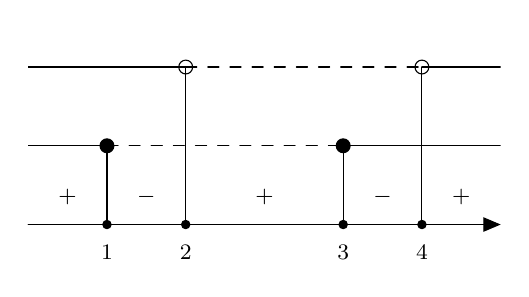
\begin{tikzpicture}[line cap=round,line join=round,>=triangle 45,x=1.0cm,y=1.0cm]
%\draw [color=black,, xstep=1.0cm,ystep=1.0cm] (-3.,-0.5) grid (3.,2.5);
\draw[->,color=black] (-3.,0.) -- (3.,0.);
;
\draw[color=black] (-1,-10pt) node {\footnotesize $2$};
\draw[color=black] (1,-10pt) node {\footnotesize $3$};
\draw[color=black] (-2,-10pt) node {\footnotesize $1$};
\draw[color=black] (2,-10pt) node {\footnotesize $4$};

\draw[color=black] (-1.5,10pt) node {\footnotesize $-$};
\draw[color=black] (1.5,10pt) node {\footnotesize $-$};
\draw[color=black] (-2.5,10pt) node {\footnotesize $+$};
\draw[color=black] (2.5,10pt) node {\footnotesize $+$};
\draw[color=black] (0,10pt) node {\footnotesize $+$};
\clip(-3.,-0.5) rectangle (3.,2.5);
\draw (-1.,2.)-- (-1.,0.);
\draw (1.,1.)-- (1.,0.);
\draw (-3.,2.)-- (-1.,2.);
\draw [dash pattern=on 4pt off 4pt] (-1.,2.)-- (2.,2.);
\draw (-3.,1.)-- (-2.,1.);
\draw (1.,1.)-- (3.,1.);
\draw (2.,2.)-- (2.,0.);
\draw (2.,2.)-- (3.,2.);
\draw (-2.,1.)-- (-2.,0.);
\draw [dash pattern=on 4pt off 4pt] (-2.,1.)-- (1.,1.);
\begin{scriptsize}
\draw  (-1.,2.) circle (2.5pt);
\draw [fill=black]  (-2.,1.) circle (2.5pt);
\draw [fill=black](1.,1.) circle (2.5pt);
\draw  (2.,2.) circle (2.5pt);
\draw [fill=black] (2.,0.) circle (1.5pt);
\draw [fill=black] (-2.,0.) circle (1.5pt);
\draw [fill=black] (1.,0.) circle (1.5pt);
\draw [fill=black] (-1.,0.) circle (1.5pt);
\end{scriptsize}
\end{tikzpicture}
\end{document}